An $N=3$ orbit, for being a triangle, will be associatd with a few ``famous'' circles: the Incircle, Circumcircle, and 9-Point Circle \cite{mw}. Denote their radii as $r$ (inradius) $R$ (circumradius) and $r_9$, respectively,  Figure~\ref{fig:radii}.

\begin{figure}[H]
    \centering
    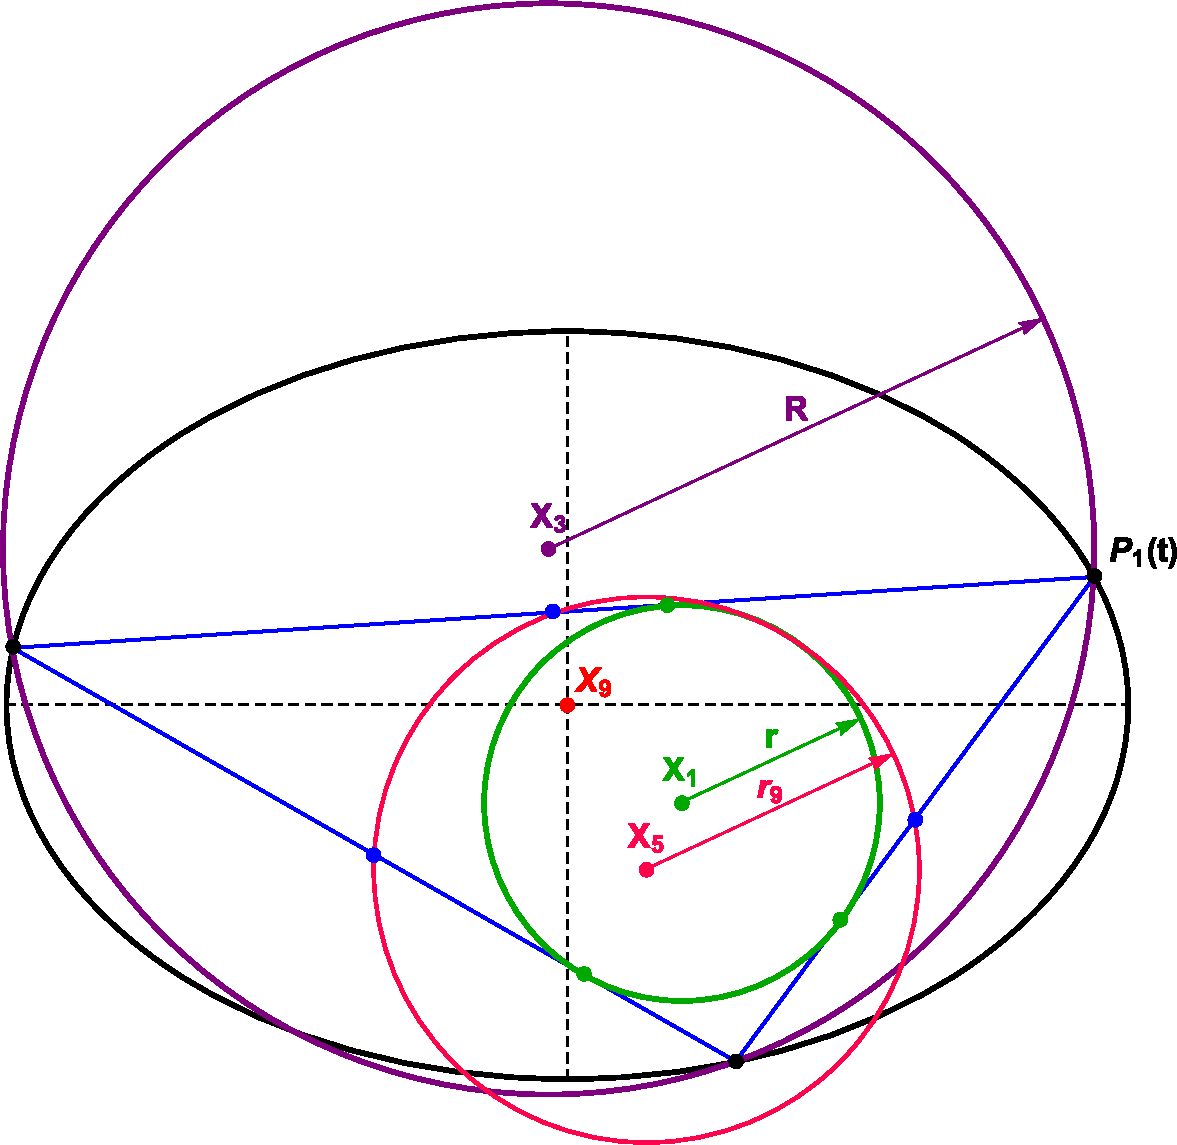
\includegraphics[width=.7\textwidth]{pics/0070_Radii.pdf}
    \caption{An orbit is shown (blue), whose leader vertex is $P_1(t)$. Shown also are its  Incircle (green), Circumcircle (purple), and 9-Point Circle (pink), with centers at $X_1$, $X_3$, and $X_5$. Their radii are the Inradius $r$, Circumradius $R$, and 9-Point Circle radius $r_9$.}
    \label{fig:radii}
\end{figure}

Inspecting the three notable radii against the parameter $t$ of $P_1$, Figure~\ref{fig:radii_plot}, one notices the known proportionality of $R=2r_9$ \cite{mw}. A remarkable fact is that $R$ is also proportional to $r$, as shown by a scatter plot Figure~\ref{fig:radii_scatter}, for any Billiard aspect ratio $a$. In fact \cite{ronaldo19a}:

\begin{equation}
\frac{r}{R}=\frac{2(\delta-1)}{(a^2-1)(\delta+a^2)}
\label{eqn:r-ov-R}
\end{equation}

Suprisingly, an alternate formula for $r/R$ has been derived \cite{dominique19,sergei19_private_circles} in terms of the perimeter $L$ and momentum $\gamma$:

\begin{equation}
    \frac{r}{R} = \gamma L - 4
    \label{eqn:rR_dominique}
\end{equation}

\begin{figure}[H]
    \centering
     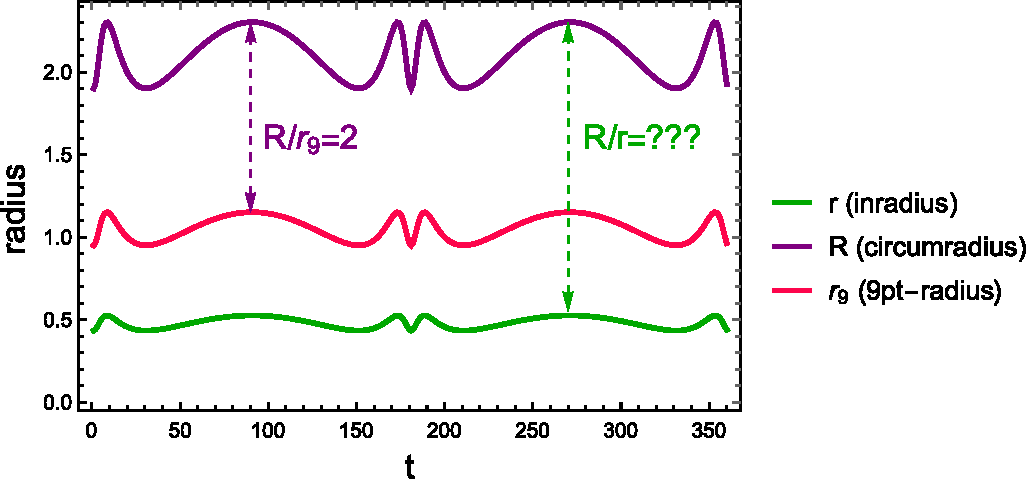
\includegraphics[width=.75\textwidth]{pics/0075_radii_plot.pdf}
    \caption{The three notable radii vs the angular parameter $t$ in $P_1(t)$. The ratio $R/r_9=2$ is known for any triangle. Suprisingly, $R/r$ is also constant over the $N=3$ orbit family.}
    \label{fig:radii_plot}
\end{figure}

\noindent Since both are constant, so must $r/R$ be, and:

\begin{theorem}
The ratio $r/R$ of Inradius to Circumradius is conserved for an $N=3$ orbit family and only depends on the Billiard's aspect ratio.
\label{obs:rovR}
\end{theorem}

As shown in Figure~\ref{fig:ratio_vs_a}, when $a=1$ (Billiard is circular), $r/R$ is maximal at $0.5$ (orbits are equilaterals). As $a\rightarrow\infty$, the ratio goes to zero. An inflection point occurs at $a\simeq{1.37}$, $r/R\simeq{.407}$, whose geometric meaning is not yet understood.

\begin{figure}[H]
    \centering
    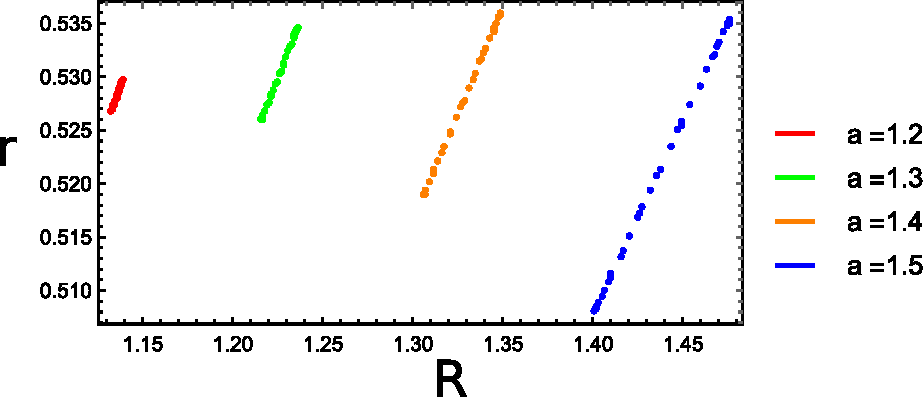
\includegraphics[width=0.75\textwidth]{pics/0080_radii_scatter.pdf}
    \caption{A scatter plot of Inradius vs Circumradius for various $t$ and various Billiard aspect ratios, showing linear dependence.}
    \label{fig:radii_scatter}
\end{figure}

\begin{figure}[H]
    \centering
    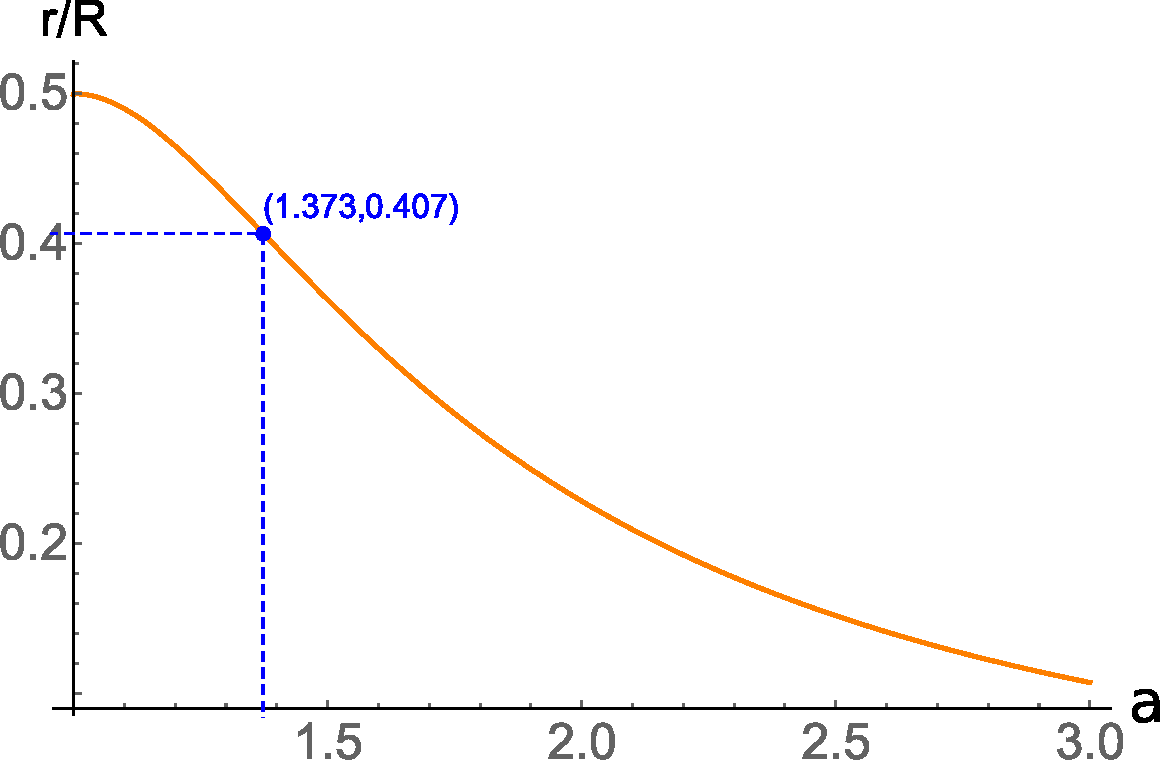
\includegraphics[width=.55\textwidth]{pics/0085_r_ov_R.pdf}
    \caption{The ratio $r/R$ as a function of the Billiard's axis ratio $a$ and an inflection point.}
    \label{fig:ratio_vs_a}
\end{figure}

\subsection{Conservation of the Sum of Cosines}

Denote $\theta_i,i=1,2,3$ the angles internal to the orbit. The following is a remarkable identity valid for any triangle \cite{johnson29}:

\begin{equation}
\sum_{i=1}^{3}{\cos\theta_i}=1+\frac{r}{R}
\label{eqn:rR_cos}
\end{equation}

Since the right-hand side is constant, so must be the sum of the cosines! These are shown against $P_1$'s parameter in Figure~\ref{fig:cosine_sum_n3}. Also shown is their their constant sum. So a corollary to Observation~\ref{obs:rovR} is:

\begin{corollary}
\label{cor8}
The sum of cosines is invariant for the $N=3$ family of orbits. 
\end{corollary}

\noindent Equations~\ref{eqn:rR_cos} and \ref{eqn:rR_dominique} imply
that the average cosine is given by:

\begin{equation}
\frac{1}{3}\sum_{i=1}^{3}{\cos\theta_i}=\frac{\gamma{L}}{3}-1
\label{eqn:rR_cos_avg}
\end{equation}

\begin{figure}[H]
    \centering
    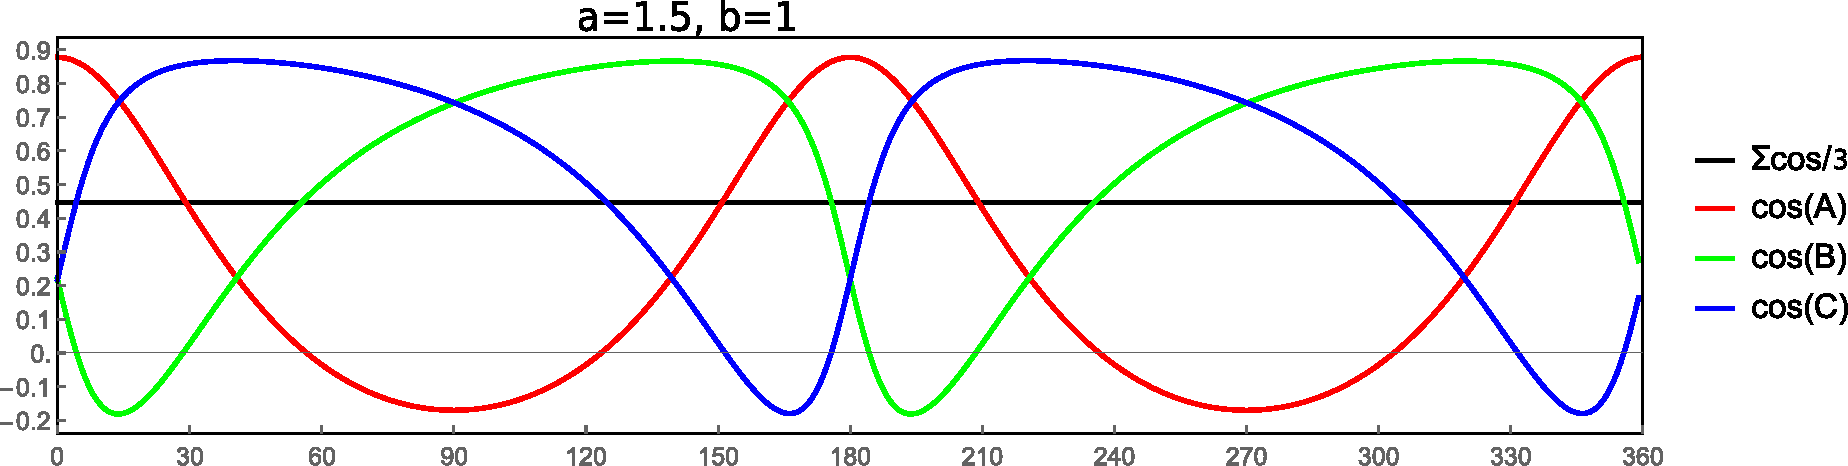
\includegraphics[width=\textwidth]{pics/0090_cosine_sum_n3.pdf}
    \caption{Cosines of each of orbit's internal angles (red, green, blue), as well as the arithmetic mean of their sum (black), showing constancy.}
    \label{fig:cosine_sum_n3}
\end{figure}

\subsection{Conservation of the Product of Excentral Cosines}

A triangle is always the Orthic of its Excentral \cite{mw}. If $\theta_i'$ are the Excentral's angles, the following is a known relation \cite{johnson29}:

\begin{equation}
\prod_{i=1}^{3}{|\cos\theta_i'|}=\frac{r}{4R}
\label{eqn:prod-cos}
\end{equation}

Let $\theta_i'$ be an angle of the Excentral Triangle opposite orbit angle $\theta_i$. It can be shown that $\theta_i'=\frac{\pi-\theta_i}{2}$, i.e., the Excentral Triangle is acute. Therefore the absolute sign in Equation~\ref{eqn:prod-cos} can be dropped. Since the right hand side of the above is constant:

\begin{corollary}
\label{cor9}
The product of cosines of Triangles Excentral to the $N=3$ orbit family is conserved.
\end{corollary}

\subsection{Conservation of Excentral-to-Orbit Area Ratio}

Let $A$ be the area of some triangle and $A_h$ the area of its Orthic. A known relation is \cite{johnson29}:

\begin{equation}
\frac{A}{A_h}=\frac{2R_h}{r_h}   
\end{equation}

Since the orbit is its Excentral's Orthic, $r/R$ constant implies:

\begin{corollary}
\label{cor10}
The Excentral-to-Orbit area ratio is constant and equal to $2R/r$.
\end{corollary}
